% Copyright (c) 2017-2020 Matematyka dla Ciekawych Świata (http://ciekawi.icm.edu.pl/)
% Copyright (c) 2017-2020 Robert Ryszard Paciorek <rrp@opcode.eu.org>
% 
% MIT License
% 
% Permission is hereby granted, free of charge, to any person obtaining a copy
% of this software and associated documentation files (the "Software"), to deal
% in the Software without restriction, including without limitation the rights
% to use, copy, modify, merge, publish, distribute, sublicense, and/or sell
% copies of the Software, and to permit persons to whom the Software is
% furnished to do so, subject to the following conditions:
% 
% The above copyright notice and this permission notice shall be included in all
% copies or substantial portions of the Software.
% 
% THE SOFTWARE IS PROVIDED "AS IS", WITHOUT WARRANTY OF ANY KIND, EXPRESS OR
% IMPLIED, INCLUDING BUT NOT LIMITED TO THE WARRANTIES OF MERCHANTABILITY,
% FITNESS FOR A PARTICULAR PURPOSE AND NONINFRINGEMENT. IN NO EVENT SHALL THE
% AUTHORS OR COPYRIGHT HOLDERS BE LIABLE FOR ANY CLAIM, DAMAGES OR OTHER
% LIABILITY, WHETHER IN AN ACTION OF CONTRACT, TORT OR OTHERWISE, ARISING FROM,
% OUT OF OR IN CONNECTION WITH THE SOFTWARE OR THE USE OR OTHER DEALINGS IN THE
% SOFTWARE.

\section{Ethernet}

% BEGIN: Warstwa sprzętowa
Od strony sprzętowej sieć składa z:
\begin{itemize}
	\item hostów stanowiących nadawców i odbiorców informacji
	\item urządzeń sieciowych pośredniczących w ich przekazywaniu, takich jak nadajniki, switche, mediakonwertery
	\item okablowania miedzianego bądź światłowodowego (jeżeli nie jest siecią bezprzewodową)
\end{itemize}

W przypadku sieci w standardzie Ethernet stosowane są 48 bitowe adresy MAC (pierwsza część identyfikuje producenta karty) oraz wspólny dla wszystkich odmian (przewodowych i bezprzewodowych) format ramki (określający położenie w ramce adresów, informacji dodatkowych oraz danych). Pakiety protokołu warstwy wyższej (np. pakiety IP wraz ich strukturą zawierającą adresy itd) z punktu widzenia ramki ethernetowej są danymi, w które ta warstwa nie wnika. Do mapowania adresów IP na adresy MAC wykorzystywany jest protokół ARP (dla IPv4) lub Neighbor Discovery (dla IPv6) - odbywa się to poprzez wysłanie ramki ethernetowej na adres rozgłoszeniowy (odbierany przez wszystkie hosty) z pytaniem o to jaki MAC adres ma host o podanym numerze IP.

Sieć ethernetowa typowo posiada strukturę wielokrotnej gwiazdy (drzewa), w węzłach której stosowane są switche. Kierują one ramki do odpowiednich gałęzi na podstawie adresu docelowego i wpisów w tablicy adresów MAC, utworzonej w oparciu o źródłowe nadawców przechodzących przez dany switch ramek. W przypadku gdy adresu docelowego nie ma w tablicy ramka kierowana jest na wszystkie porty switcha z wyjątkiem tego na którym została odebrana. W taki sposób zawsze są też przesyłane ramki wysyłane na adres rozgłoszeniowy (bradcast).

\begin{teacherOnly} % prehistoria czyli hub'y
Można wspomnieć że dawniej funkcję switchy pełniły (dzisiaj już nie spotykany) mostek (bridge) będący w zasadzie switchem o dwóch gniazdach.
Natomiast do łączenia kabli wykorzystywany był (także już nie spotykany) hub (koncentrator) który zapewniał że sygnał nadawany przez dowolny z hostów do niego podłączonych był odbierany przez wszystkie inne (poza nim samym) oraz wzmacniał sygnał. Występował także regenerator (repeater) wzmacniający sygnał i umożliwiający przekroczenie ograniczenia 100m.

Najprostszy hub to w zasadzie drabinka oporników zapewniająca że po pełnym obiegu mamy oporność nieskończonej linii (100omów).
Można obyć się nawet bez żadnego huba, a jedynie z wykorzystaniem zwykłego trójnika (tutaj komputery wpięte w gniazdka trójnika się nie widzą - widzą tylko ten po drugiej stronie, a w komunikacji dużą rolę odgrywa protokół CSMA/CD).
\end{teacherOnly}

W przewodowych sieciach Ethernet wykrywaniem zajętości medium transmisyjnego oraz wykrywaniem kolizji zajmuje się protokół CSMA/CD (Carrier Sense Multiple Access with Collision Detection - wielodostęp z rozpoznawaniem stanu kanału oraz wykrywaniem kolizji). Przed rozpoczęciem nadawania stacja musi sprawdzić czy medium jest wolne, jeżeli tak może zacząć nadawać, jeżeli dwie stacje zaczną nadawać równocześnie zostaje to wykryte, obie przerywają nadawanie i wznawiają po losowym czasie. Jednak ze względu na stosowanie głównie połączeń punkt-punkt full-duplex (osobne przewody do nadawania i osobne do odbioru), co ogranicza tzw. domenę kolizji do pojedynczego hosta, protokół ten nie odgrywa tutaj szczególnie istotnej roli.

\subsection{Ramka}

\begin{figure}[h!]
	\begin{center}\hspace{-4.0cm}\begin{adjustbox}{scale=0.64}
		\inputFileContent{booklets-sections/network/ilustracje/40-ethernet.tex}
	\end{adjustbox}\end{center}\vspace{-0.5cm}
\end{figure}

Przyglądając się przedstawionej ramce ethernetowej warto zauważyć iż długość przesyłanych w niej danych musi zawierać się w zakresie od 46 do 1500 bajtów.
Ograniczenia te wynikają ze specyfikacji elektrycznej ethernetu i protokołu CSMA/CD.
Dolne ograniczenie łatwo jest wyeliminować dopełniając pole dane jakimiś wartościami. Jednak górne ogranicza nam maksymalną długość pakietu IP przesyłanego taką ramką, wyznaczając wartość MTU (Maximum Transmission Unit).
W różnych sieciach L2, wartość MTU może być różna. Nawet w Ethernecie istnieje możliwość zwiększenia MTU dla danej sieci (jeżeli sprzęt w tej sieci wspierają większe ramki – \textit{jumbo frames}), jak również zmniejszenia MTU na danym interfejsie (np. gdy ruch z niego będzie przesyłany dalej łączem o mniejszym MTU).

Problem niedopasowania pakietu IP do MTU można rozwiązać na dwa sposoby – nie generować pakietów większych niż najmniejsze MTU na trasie (mechanizm detekcji MTU) lub dzielić większe pakiety na mniejsze w trakcie przesyłu (mechanizm fragmentacji)  . Można się spotkać z obydwoma tymi podejściami, aczkolwiek raczej unika się fragmentacji pakietów.

\subsection{VLANy, bonding, ...}

Ethernet pozwala na wirtualne podzielenie pojedynczej sieci lokalnej na wiele niezależnych (nie komunikujących się ze sobą w warstwie ethernetu) sieci, nazywanych VLAN. Działanie tego mechanizmu opiera się na zastosowaniu zarządzalnych switchy, które programowo mogą być dzielone na części zapewniające separację ruchu poszczególnych VLANów. Ponadto wybrane porty takiego switcha mogą być przypisane do różnych części (celem udostępnienia do innego switcha lub hosta kilku sieci wirtualnych), w takim przypadku do ramek ethernetowych wysyłanych tym portem dodawana jest informacja do którego VLANu należą (dwu bajtowy numer), a w przypadku ramek otrzymywanych na podstawie tego numeru odbywa się ich kierowanie do odpowiedniej "części" przełącznika (mówimy o VLANach tagowanych). Możliwe jest aby jeden wybrany VLAN na takim porcie był nie tagowany (do jego ramek nie będzie dodawany numer, a otrzymywane pakiety bez numeru będą kierowane do niego.

Ethernet pozwala również na grupowanie kilku portów w jeden port wirtualny (tzw port trunking / bonding) celem zwiększenia przepustowości lub niezawodności łącza. A dzięki zastosowaniu w różnych typach sieci ethernet tego samego formatu ramki możliwe jest też stosunkowo proste zmienianie medium transmisyjnego (np. z kabla miedzianego na światłowód) z użyciem media-konwerterów.
% END: Warstwa sprzętowa


\subsection{Kable}

Sieć ethernetowa wykorzystuje 8 żyłowe kable złożone z 4 par. Najpopularniejszym przewodem jest kabel UTP kategorii 5e, czyli nieekranowana skrętka pozwalająca na pracę z częstotliwością 100 MHz. W przypadku instalacji okablowania strukturalnego często stosowane są wyższe kategorie okablowania a także kable dodatkowo ekranowane. Ekran może obejmować osobno każdą parę, jak też może być wspólny dla całego przewodu, może być wykonany z folii lub siatki. Np. SF/FTP oznacza kabel z ekranem z siatki i folii (SF/), gdzie dodatkowo każda para jest ekranowana folią (FTP).

W ramach poszczególnych par realizowana jest transmisja różnicowa, czyli istotne jest napięcie pomiędzy przewodami w parze, a nie napięcie na danym przewodzie (w odniesieniu do jakiegoś zewnętrznego poziomu odniesienia).
Standard 100Mb/s (dokładniej 100BASE-TX) wykorzystuje jedynie dwie pary przewodów, standard 1Gb/s (1000BASE‑T) wykorzystuje wszystkie 4 pary przewodów.
Długość kabla pomiędzy dwoma urządzeniami nie powinna przekraczać 100 m.
Wykorzystywanie skręconych par przewodów (jeden skręt na 6-10 cm kabla) ma na celu eliminację zakłóceń transmisji - (w uproszczeniu) zakłócenia wchodzą tak samo na oba przewody i różnica miedzy nimi nie zmienia się.

Kable zakańczane są gniazdami bądź wtykami typu RJ-45 montowanymi według jednego z dwóch schematów kolorystycznych: EIA/TIA 568A lub 568B.
Pierwotnie (dla sieci 100Mb/s lub starszych) użycie różnych standardów na obu końcach kabla służyło stworzeniu kabla skrosowanego\footnote{Połączenie takie przy jednakowych urządzeniach, gdzie nadajnik i odbiornik trafia zawsze na te same piny, zamieniało na kablu nadajnik z odbiornikiem, umożliwiając transmisje między nimi. Aktualnie zdecydowana większość urządzeń obsługuje protokół \emph{Auto MDI-X}, który umożliwia automatyczne ustalenie na których pinach odbywa się nadawanie, a na których odbiór. W rzadkich przypadkach konieczne może być jednak zastosowanie kabla skrosowanego}.

\vspace{0.3cm}\noindent
\begin{minipage}{0.47\textwidth}
\begin{center}
{\noindent\large\bfseries EIA/TIA 568A}

{\noindent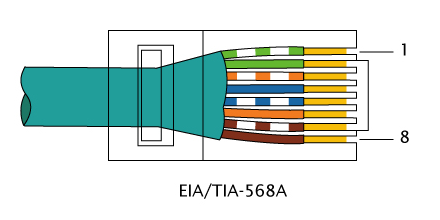
\includegraphics[width=0.7\textwidth,clip=true,trim={0, 4.5mm, 0, 0}]{RJ-45_TIA-568A_Right.png}}
\end{center}
\vspace{-0.3cm}

Kolejność przewodów we wtyczce/gnieździe:
\begin{enumerate}
	\item biało-zielony
	\item zielony
	\item biało-pomarańczowy
	\item niebieski
	\item biało-niebieski
	\item pomarańczowy
	\item biało-brązowy
	\item brązowy
\end{enumerate}
\end{minipage}
\hfill
\begin{minipage}{0.47\textwidth}
\begin{center}
{\noindent\large\bfseries EIA/TIA 568B}

{\noindent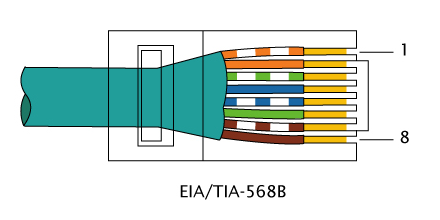
\includegraphics[width=0.7\textwidth,clip=true,trim={0, 4.5mm, 0, 0}]{RJ-45_TIA-568B_Right.png}}
\end{center}
\vspace{-0.3cm}

Kolejność przewodów we wtyczce/gnieździe:
\begin{enumerate}
	\item biało-pomarańczowy
	\item pomarańczowy
	\item biało-zielony
	\item niebieski
	\item biało-niebieski
	\item zielony
	\item biało-brązowy
	\item brązowy
\end{enumerate}
\end{minipage}
\vspace{0.3cm}

Wtyczki RJ-45 są wtyczkami zaciskanymi na przewodzie (bez konieczności odizolowywania żył). Gniazda RJ-45 najczęściej wykonywane są ze złączem typu IDC (Insulation Displacement Connector, KRONE/LSA) służącym do podłączenia przewodu również bez konieczności odizolowywania poszczególnych żył.
